%=========================================================================
% sec-tuning
%=========================================================================

\section{Tuning the Convolutional Neural Network}
\label{sec-tuning}

\subsection{Manual Vectorization}
\label{sec-tuning-vectorization}

%=========================================================================
% fig-tuning-vectorization-convolution.tex
%=========================================================================

\begin{figure}[h]

  \centering
  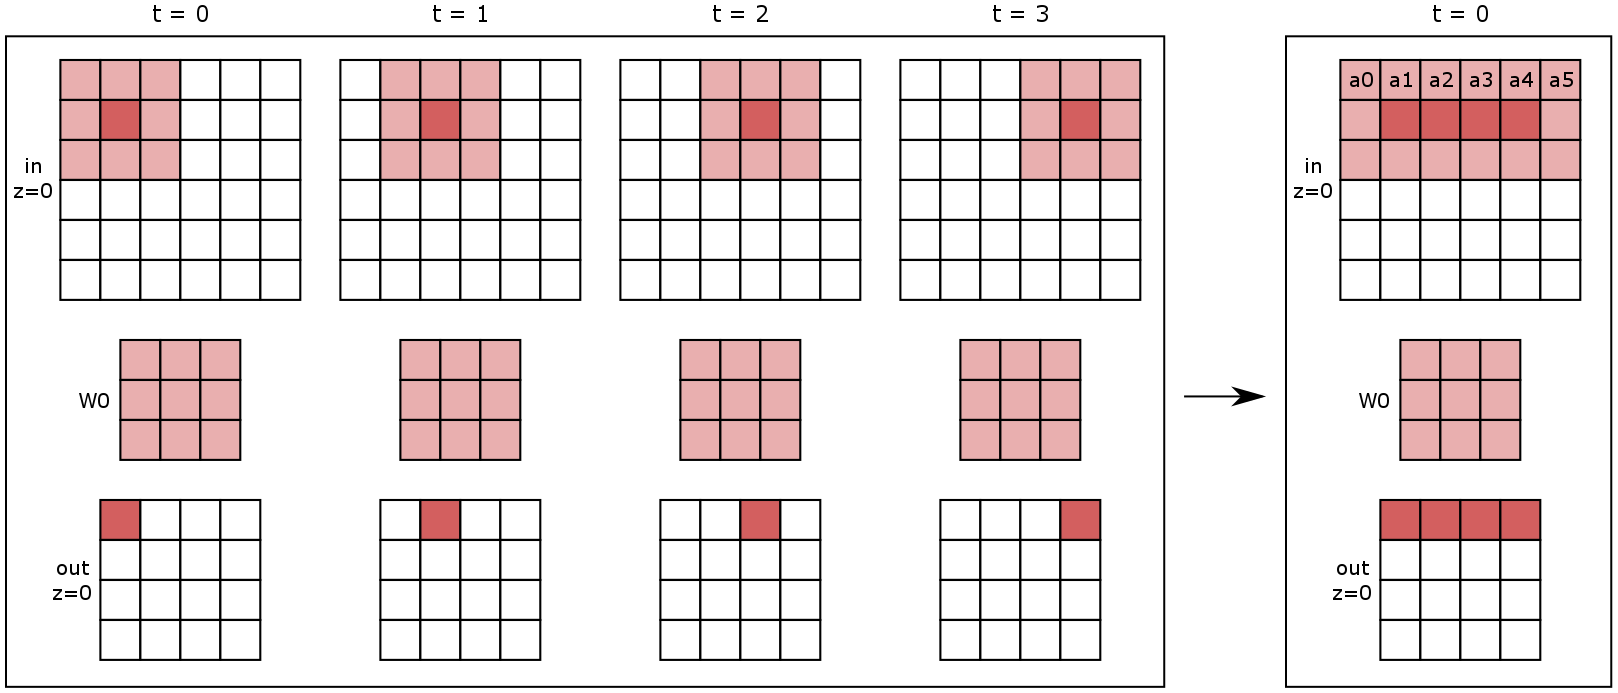
\includegraphics[width=0.9\tw]{fig-tune-vector-convolution.svg.pdf}

  \caption{\textbf{Vectorization Strategy for Convolutional Layer --} A
    6x6x1 input is convolved with a 3x3x1 filter to produce a 4x4x1 slice
    of the output. For simplicity, only one filter and the computation
    required for a single slice is shown. The box on the left illustrates
    the scalarized approach that takes four computational timesteps to
    calculate the first row of the output. The box on the
    right illustrates the vectorized approach that takes a single
    computational timestep to perform the same computations.}

  \label{fig-tuning-vectorization-convolution}

\end{figure}

%=========================================================================
% fig-tuning-vectorization-convolution-access.tex
%=========================================================================

\begin{figure}[h!]

  \centering
  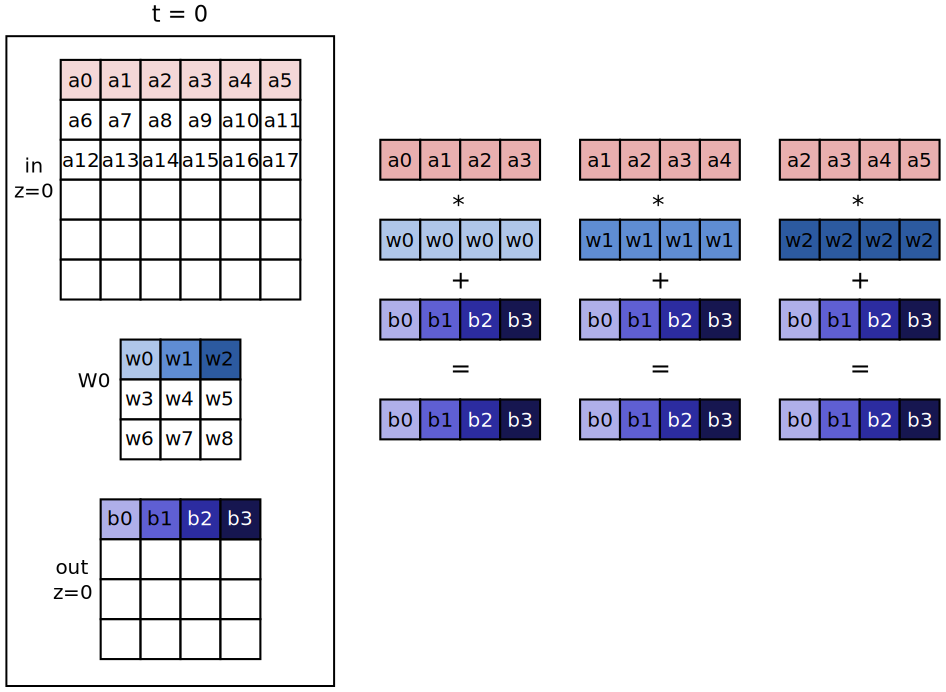
\includegraphics[width=0.5\tw]{fig-tune-vector-convolution-access.svg.pdf}

  \caption{\textbf{Memory Access Pattern for Convolutional Layer --}
    Breakdown of the vector operations required to compute the first row
    of the output in a convolutional layer. Each element in the vector
    corresponds to a separate element in the output. Contiguous elements
    in the input are loaded into a vector register and multiplied with
    the same weight broadcasted to another vector register. The partial
    products are accumulated to the output elements until all weights
    have been applied. Note that the accumulation can be performed in a
    single vector register without intermediate stores.}

  \label{fig-tuning-vectorization-convolution-access}

\end{figure}

%=========================================================================
% fig-tuning-vectorization-pooling.tex
%=========================================================================

\begin{figure}[t]

  \centering
  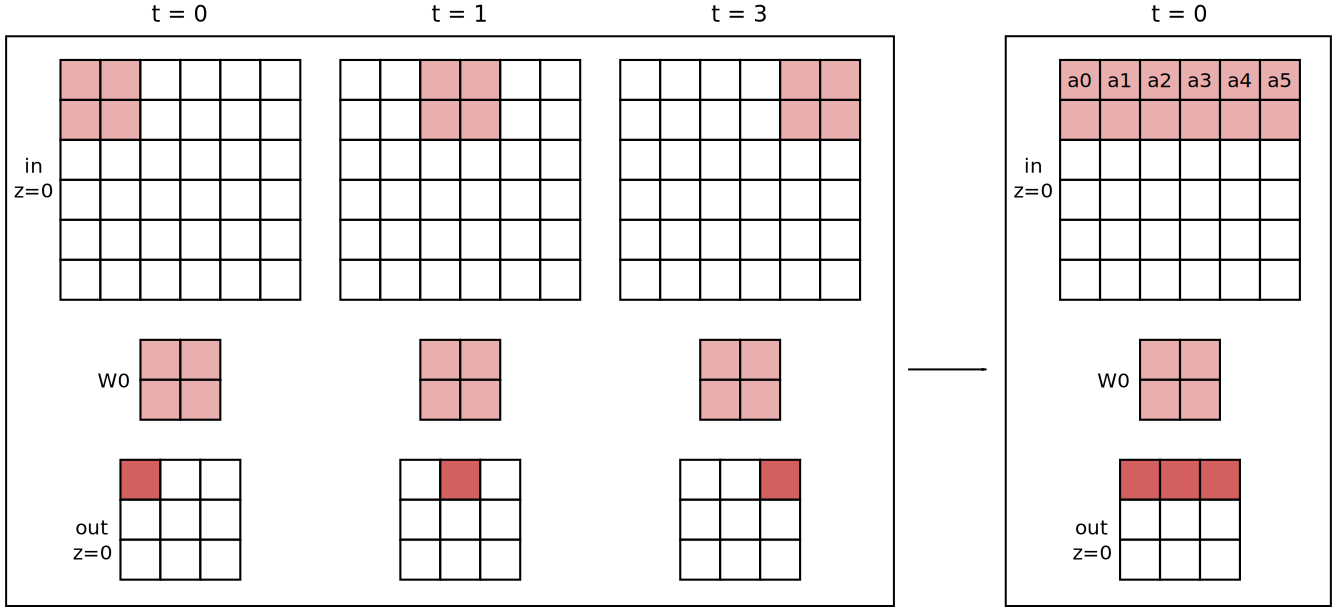
\includegraphics[width=0.9\tw]{fig-tune-vector-pooling.svg.pdf}

  \caption{\textbf{Vectorization Strategy for Pooling Layer --} A 6x6x1
    input is downsampled using a 2x2x1 filter to produce a 3x3x1 slice of
    the output. The box on the left illustrates the scalarized approach
    that takes three computational timesteps to calculate the first row
    of the output. The box on the right illustrates the vectorized
    approach that takes a single computational timestep to perform the
    same computations.}

  \label{fig-tuning-vectorization-pooling}

\end{figure}

%=========================================================================
% fig-tuning-vectorization-pooling-access.tex
%=========================================================================

\begin{figure*}[t]

  \centering
  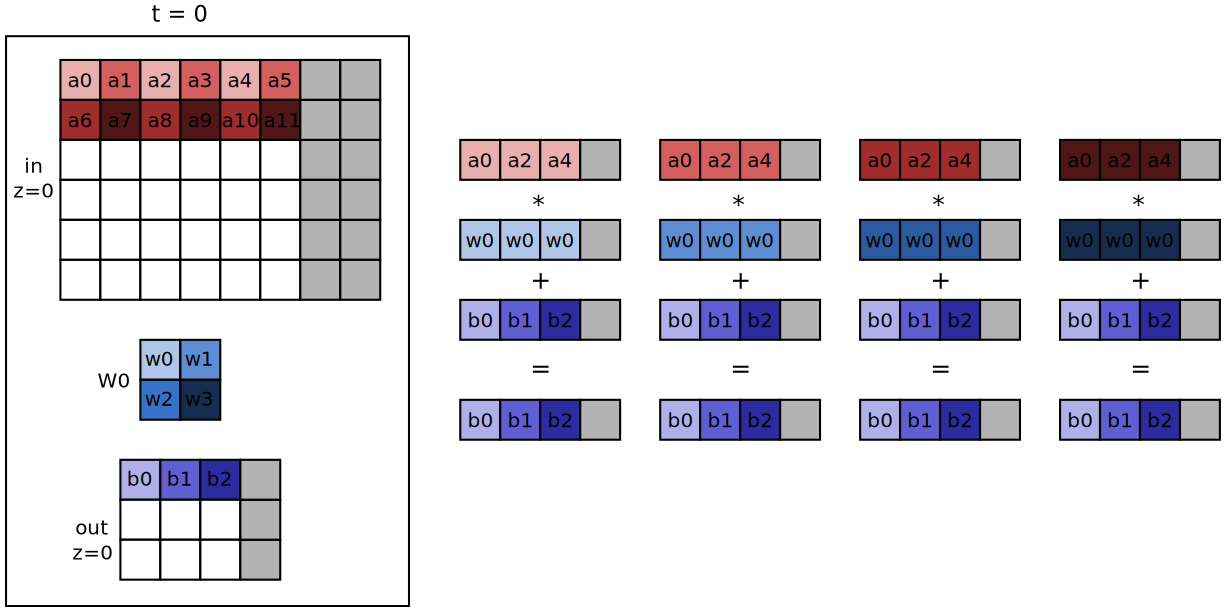
\includegraphics[width=0.9\tw]{fig-tune-vector-pooling-access.svg.pdf}

  \caption{\textbf{Memory Access Pattern for Pooling Layer --}
    Breakdown of the vector operations required to compute the first row
    of the output in a pooling layer. Each element in the vector
    corresponds to a separate element in the output. A strided load is
    used to load the input elements since the filter is applied with a
    non-unit stride for pooling layers. Otherwise, the same multiply-add
    accumulation occurs as in the convolutional layer. This example shows
    an example of padding the memory layout of the input and output so
    that vector loads/stores do not access unallocated memory.}

  \label{fig-tuning-vectorization-pooling-access}

\end{figure*}


As we learned from previous assignments in the course, it is necessary to
maximize and leverage opportunities for vectorization in order to achieve
any speedups when offloading to the MIC. This is because although the MIC
has many more cores than the compute nodes, each core is actually
significantly simpler than those in the compute nodes. The advantage of
the MIC heavily depends on the utilization of its wider (512b) SIMD
pipelines.

We first analyzed the efficacy of the auto-vectorization of the
baseline. Even using ICC, the reports showed a disappointing level of
vectorization--essentially only the initialization loops were being
vectorized. This is likely due to the baseline being written in C++ (as
we saw with the shallow water assignment), especially the gratuitous use
of templating for defining the connectivity between inputs and outputs in
each layer. As such, we manually vectorized the most performance-critical
functions of the code for both the compute nodes and the MIC using AVX2
and AVX-512 intrinsics, respectively. It is worth noting that although
the baseline did have some level of manual vectorization, it was limited
to the fully connected layers, which is the least performance-critical
computational layer in the CNN. The performance-critical functions turned
out to be the \texttt{forward\_propagation()} and
\texttt{backward\_propagation()} functions of the convolutional and
pooling layers that compose a majority of the CNN pipeline.

Figure~\ref{fig-tuning-vectorization-convolution} shows the vectorization
strategy used for the forward propagation in the convolutional layer. For
simplicity, this example shows a 6x6x1 input being convolved with a 3x3x1
filter (one of $N$ filters) to produce a 4x4x1 slice of the 4x4x$N$
output. The left shows the convolutions required to compute the first row
of the output. Each element in the output is computed by multiplying the
weights in the filter with the corresponding elements in the input and
accumulating the partial product for all weights in the filter. The key
observation here is that the same weights need to be applied to
consecutive elements in the input to calculate the corresponding outputs.
This memory access pattern can be seen in
Figure~\ref{fig-tuning-vectorization-convolution-access}. We exploit this
pattern by vectorizing across the elements in the \emph{same row of the
  output}. For example,
in order to compute the output vector ${b0,b1,b2,b3}$, the weight $w0$
needs to be applied to the input vector ${a0,a1,a2,a3}$. Although the
figure only shows the first three weights being applied, all nine weights
must be applied before storing the result back to the output in
memory. The operations required for computing a vector of output elements
using an $N$x$N$ filter are $N^2$ vector loads, $N^2$ vector
multiply-adds, and one vector store.

\subsection{Memory Layout}
\label{sec-tuning-memory}

So far we have been assuming that the manual vectorization described
above operates on unaligned inputs/outputs in memory. Although unaligned
vector loads/stores are available, at least on the compute nodes, they
are less preferable compared to their aligned counterparts for
performance. The baseline uses C++ standard vector data structures which
do not guarantee alignment, so we allocated separate per-layer per-thread
C arrays with forced vector alignment. When either the forward or
backward propagation functions for a layer is called, the input is copied
to the alignment scratchpad from which all further computation
references, and the output is stored in the aligned scratchpad. Once all
elements in the output are computed, the data in the aligned scratchpad
is copied to the default unaligned data structure.

The inputs/outputs are arranged in row-major order in memory where the
$X$x$Y$x$Z$ dimensions are flattened into a 1D array. All filters are
also flattened into a 1D array (i.e., $N$x$N$x$Z$x$M$, for $M$
filters). If the filter dimensions are less than the input dimensions,
which is the common case, we cannot naively process consecutive vectors'
worth of elements in the output in this flattened 1D array. This is
because the unit-stride access we saw before only holds for elements in
the same \emph{row} of the output (i.e., $X$-dimension), so we cannot
allow a vector to span multiple rows. It follows then, that the aligned
data structures needed to be padded to a multiple of the vector length on
a \emph{per-row} basis as shown in
Figure~\ref{fig-tuning-vectorization-pooling-access}. For pooling layers,
this padding needs to a multiple of the vector length times the stride of
the pooling filter. As such, the innermost loop in the propagation
functions iterate across the elements in the current row in vector-wide
chunks. If the dimensions are not evenly divisible by the vector length,
then the last iteration will safely access the padding instead of
corrupting the next row or raising a segfault.

This alternative memory layout allows us to utilize the more efficient
aligned vector loads/stores, but unfortunately not always. The
problematic case is for the computations that use a weight that is not
the first element in the filter's row. An example of this is the second
column of computation in
Figure~\ref{fig-tuning-vectorization-convolution-access}. Even if the
input data structure is aligned, if the base address of a vector load is
not on a vector-aligned boundary as in the example, we cannot perform an
aligned load. This can easily be addressed by using intrinsics for
unaligned vector loads/stores on the compute nodes, but it is not as
simple for the MIC. It seems that although the AVX-512 ISA states an
unaligned variant exists, the version of ICC used in the course does not
seem to recognize it. It is possible that the unaligned variant was only
included for the latest MIC model, Knight's Landing. Another potential
solution was to use a combination of the \texttt{loadunpacklo/hi} and
\texttt{packstorelo/hi} intrinsics to emulate an unaligned load/store
using two aligned loads/stores. Although these intrinsics are clearly
defined in the Knight's Corner manual (exact same model as the MIC used
in the course), the compiler did not seem to recognize it. Due to the
challenges with the compiler, the last resort for enabling unaligned
loads/stores on the MIC was to use gather/scatter intrinsics with the
stride set to one. This is not desirable since gathers/scatters are
effectively equivalent to doing a separate scalar load for every element
in the vector, but it was the only option left.

The issue with unaligned loads is a consequence of vectorizing
computation across consecutive elements within a row of the output. This
would have been avoided by using an alternative vectorization strategy
that vectorizes across the same (i,j)-th element in each slice of the
output. Ironically, this was the first vectorization strategy we
attempted, but we aborted because this would have required us to change
the way the data was laid out in memory for all major data structures in
the code. Specifically, all data structures would have had to be
converted to $Z$-major order (instead of $X$-major order), so that we
could do vector loads across the $Z$-dimension.
